\chapter{Householder Triangularization}
The other principal method for computing QR factorizations is Householder triangularization, which is numerically more stable than Gram-Schmidt orthogonalization, though it lacks the latter's applicability as a basis for iterative methods. The Householder algorithm is a process of "orthogonal triangularization," making a matrix triangular by a sequence of unitary matrix operations.

\section{Householder and Gram-Schmidt} 
The GS iteration applies a succession of elementary triangular matrices $R_k$ on the right of $A$:
\[
    A \underbrace{R_1 R_2 \cdots R_n}_{\hat{R}^{-1}}=\hat{Q}.
\]
In contrast, the Householder method applies a succession of elementary unitary matrices $Q_k$ on the left of $A$, 
\[
    \underbrace{Q_n \cdots Q_2 Q_1}_{Q^*} A=R. 
\]
The two methods can be summerized as the follows: 
\begin{itemize}
    \item GS: triangular orthogonalization. 
    \item Householder: orthogonal triangularizaion. 
\end{itemize}

\section{Triangularization by Introducing Zeros} 
The idea of the Householder is to introduce zeros below the diagonal in the $k$th column while preserving all the zeros previously introduced. 
%────────────────────────────────────────
\begin{figure}[H]
    \centering
    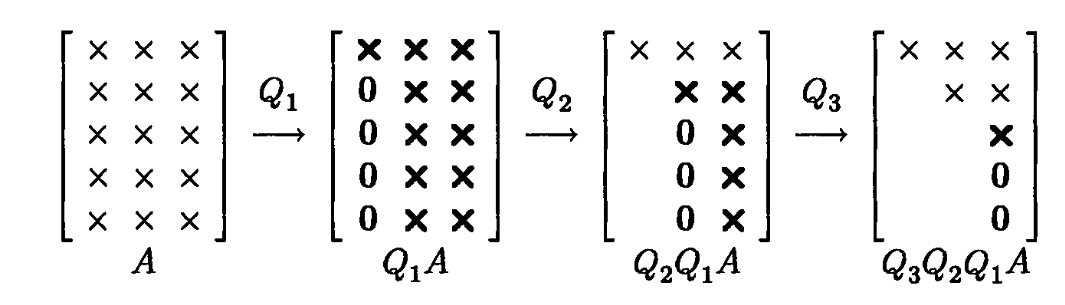
\includegraphics[width=0.8\textwidth]{figures/10-1.png}
    \caption{One example in $\RR^{5\times 3}$}
\end{figure}
%────────────────────────────────────────
In fact, $Q_k$ operates on rows $k,\ldots ,m$. At the beginning of step $k$, there is a block of zeros in the first $k-1$ columns of these rows. 

\section{Householder Reflectors} 
Each $Q_k$ is chosen to be a unitary matrix of the form: 
\[
    Q_k=\left[\begin{array}{ll}
        I & 0 \\
        0 & F
        \end{array}\right],
\]
where $I$ is the $(k-1) \times(k-1)$ identity and $F$ is an $(m-k+1) \times(m-$ $k+1)$ unitary matrix. Multiplication by $F$ must introduce zeros into the $k$th column. The householder algorithm chooses $F$ to be a particular matrix called a Householder reflector.  Suppose, at the beginning of step $k$, the entries $k, \ldots, m$ of the $k$ th column are given by the vector $x \in \mathbb{C}^{m-k+1}$. To introduce the correct zeros into the $k$ th column, the Householder reflector $F$ should effect the following map:
$$
x=\left[\begin{array}{c}
\times \\
\times \\
\times \\
\vdots \\
\times
\end{array}\right] \quad \longrightarrow \quad F x=\left[\begin{array}{c}
\|x\| \\
0 \\
0 \\
\vdots \\
0
\end{array}\right]=\|x\| e_1 .
$$
The idea for accomplishing this is indicated in Figure 10.2. The reflector $F$ will reflect the space $\mathbb{C}^{m-k+1}$ across the hyperplane $H$ orthogonal to $v=\|x\| e_1-x$. 

%────────────────────────────────────────
\begin{figure}[H]
    \centering
    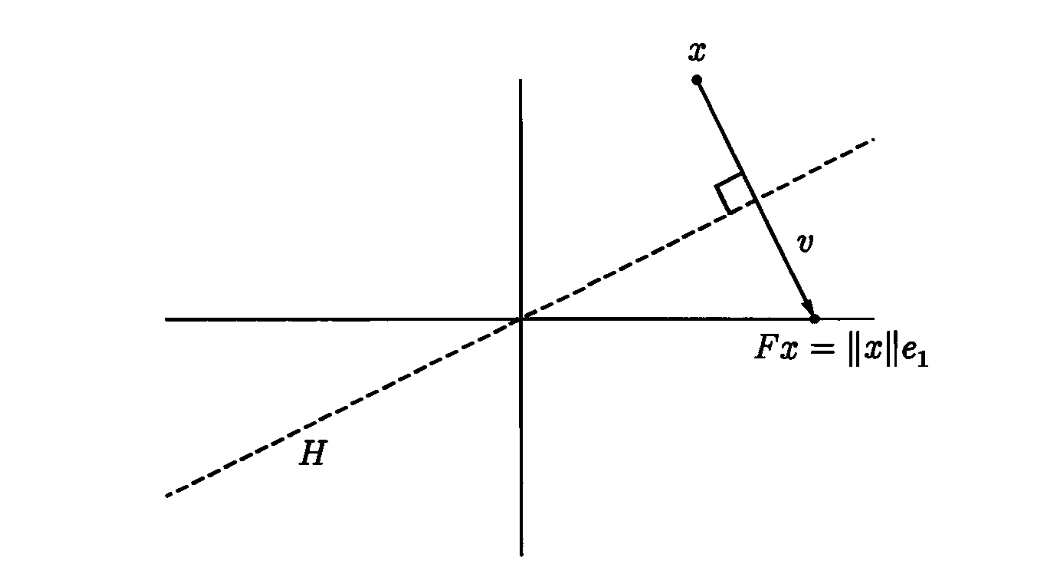
\includegraphics[width=0.8\textwidth]{figures/10-2.png}
    \label{fig 10-2}
    \caption{A Householder reflection} 
\end{figure}
%────────────────────────────────────────

The formula for this reflection can be derived as follows. We know that for any $y\in \CC^m$, the vector: 
\[
    P y=\left(I-\frac{v v^*}{v^* v}\right) y=y-v\left(\frac{v^* y}{v^* v}\right)
\]
is the orthogonal projection of $y$ onto the space $H$. To reflect $y$ across $H$, we must not stop at this point; we must go exactly twice as far in the same direction. The reflection Fy should therefore be
$$
F y=\left(I-2 \frac{v v^*}{v^* v}\right) y=y-2 v\left(\frac{v^* y}{v^* v}\right) \text {. }
$$
Hence the matrix $F$ is
$$
F=I-2 \frac{v v^*}{v^* v}
$$
Note that the projector $P$ (rank $m-1$ ) and the reflector $F$ (full rank, unitary) differ only in the presence of a factor of 2.

\section{The Better of Two Reflectors} 
In fact, there are many Householder reflections that will introduce the zeros needed. The vector $x$ can be reflected to $z\|x\| e_1$, where $z$ is any scalar with $|z|=1$. In the complex case, there is a circle of possible reflections, and even in the real case, there are two alternatives, represented by reflections across two different hyperplanes, $H^{+}$and $H^{-}$, as illustrated in Figure 10.3.
%────────────────────────────────────────
\begin{figure}[H]
    \centering
    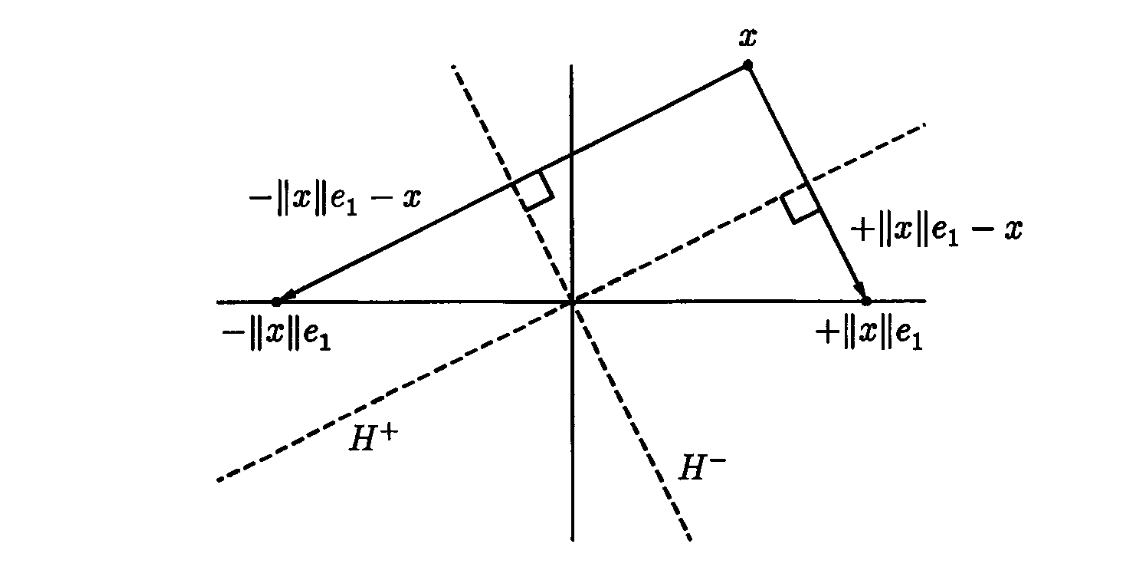
\includegraphics[width=0.8\textwidth]{figures/10-3.png}
    \label{fig 10.3}
    \caption{Two possible reflections}
\end{figure}
%────────────────────────────────────────
Mathematically, either choice of sign is satisfactory. However, this is a case where the goal of numerical stability-insensitivity to rounding errorsdictates that one choice should be taken rather than the other. For numerical stability, it is desirable to reflect $x$ to the vector $z\|x\| e_1$ that is not too close to $x$ itself. To achieve this, we can choose $z=-\operatorname{sign}\left(x_1\right)$, where $x_1$ denotes the first component of $x$, so that the reflection vector becomes $v=-\operatorname{sign}\left(x_1\right)\|x\| e_1-x$, or 
\[
    v=\operatorname{sign}\left(x_1\right)\|x\| e_1+x. 
\]
If $x_1=0$, we impose that $\sign(x_1)=1$. 

\section{The Algorithm} 
We now formulate the whole Householder algorithm. If $A$ is a matrix, we define $A_{i: i^i, j: j^{\prime}}$ to be the $\left(i^{\prime}-i+1\right) \times\left(j^{\prime}-j+1\right)$ submatrix of $A$ with upper-left corner $a_{i j}$ and lower-right corner $a_{i^{\prime}, j^{\prime}}$. In the special case where the submatrix reduces to a subvector of a single row or column, we write $A_{i, j: j^{\prime}}$ or $A_{i: i^{\prime}, j}$, respectively.

\begin{algorithm}[H]
    \caption{Householder QR factorization}
    \label{Algo 10.1}
    \For{$k=1$ \KwTo $n$}{
    $ x=A_{k: m, k} $\; 
    $v_k=\operatorname{sign}\left(x_1\right)\|x\|_2 e_1+x$\;
    $v_k=v_k /\left\|v_k\right\|_2$ \;
    $A_{k: m, k: n}=A_{k: m, k: n}-2 v_k\left(v_k^* A_{k: m, k: n}\right)$\;
    }
\end{algorithm}

\section{Applying or Forming $Q$} 
The \autoref{Algo 10.1} can get $R$ easily.  However, we still have to form the matrix $Q$. Constructing $Q$ or $\hat{Q}$ takes additional work, and in many applications, we can avoid this by working directly with the formula
$$
Q^*=Q_n \cdots Q_2 Q_1
$$
or its conjugate
$$
Q=Q_1 Q_2 \cdots Q_n. 
$$ 
In fact, we only need to the matvec $Q^*b$ or $Qx$. The algorithms are:

\begin{algorithm}[H]
    \caption{Implicit Calculation of a Product $Q^*b$}
    \label{Algo 10.2}
    \For{$k=1$ \KwTo $n$} {
        $b_{k: m}=b_{k: m}-2 v_k\left(v_k^* b_{k: m}\right)$
    }
\end{algorithm}

\begin{algorithm}[H]
    \caption{Implicit Calculation of a Product $Qx$}
    \label{Algo 10.3}
    \For{$k=n$ \KwTo $1$} {
        $x_{k: m}=x_{k: m}-2 v_k\left(v_k^* x_{k: m}\right)$
    }
\end{algorithm}
The work involved in either of these algorithms is of order $O(m n)$, not $O\left(m n^2\right)$ as in \autoref{Algo 10.1} (see below).

Sometimes, of course, one may wish to construct the matrix $Q$ explicitly. This can be achieved in various ways. We can construct $Q I$ via Algorithm 10.3 by computing its columns $Q e_1, Q e_2, \ldots, Q e_m$. Alternatively, we can construct $Q^* I$ via Algorithm 10.2 and then conjugate the result. A variant of this idea is to conjugate each step rather than the final product, that is, to construct $I Q$ by computing its rows $e_1^* Q, e_2^* Q, \ldots, e_m^* Q$. Of these various ideas, the best is the first one, based on \autoref{Algo 10.3}. The reason is that it begins with operations involving $Q_n, Q_{n-1}$, and so on that modify only a small part of the vector they are applied to; if advantage is taken of this sparsity property, a speed-up is achieved.

If only $\hat{Q}$ rather than $Q$ is needed, it is enough to compute the columns $Q e_1, Q e_2, \ldots, Q e_n$.

\section{Operation Count} 
The work involved in \autoref{Algo 10.1} is dominated by the innermost loop,
$$
A_{k: m, j}-2 v_k\left(v_k^* A_{k: m, k}\right)
$$
If the vector length is $l=m-k+1$, this calculation requires $4 l-1 \sim 4 l$ scalar operations: $l$ for the subtraction, $l$ for the scalar multiplication, and $2 l-1$ for the dot product. This is $\sim 4$ flops for each entry operated on.

We may add up these four flops per entry by geometric reasoning. Each successive step of the outer loop operates on fewer rows, because during step $k$, rows $1, \ldots, k-1$ are not changed. Furthermore, each step operates on fewer columns, because columns $1, \ldots, k-1$ of the rows operated on are zero and are skipped. Thus the work done by one outer step can be represented by a single layer of the following solid:
%────────────────────────────────────────
\begin{figure}[H]
    \centering
    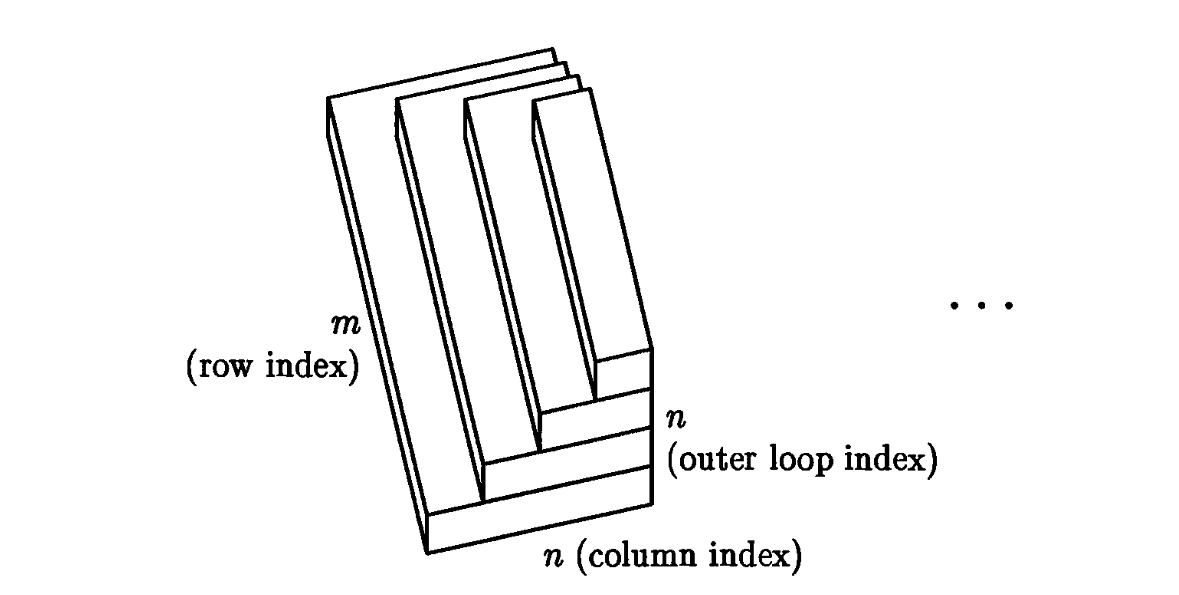
\includegraphics[width=0.8\textwidth]{figures/10-4.png}
\end{figure}
%────────────────────────────────────────
This can be divide into two pieces: 

%────────────────────────────────────────
\begin{figure}[H]
    \centering
    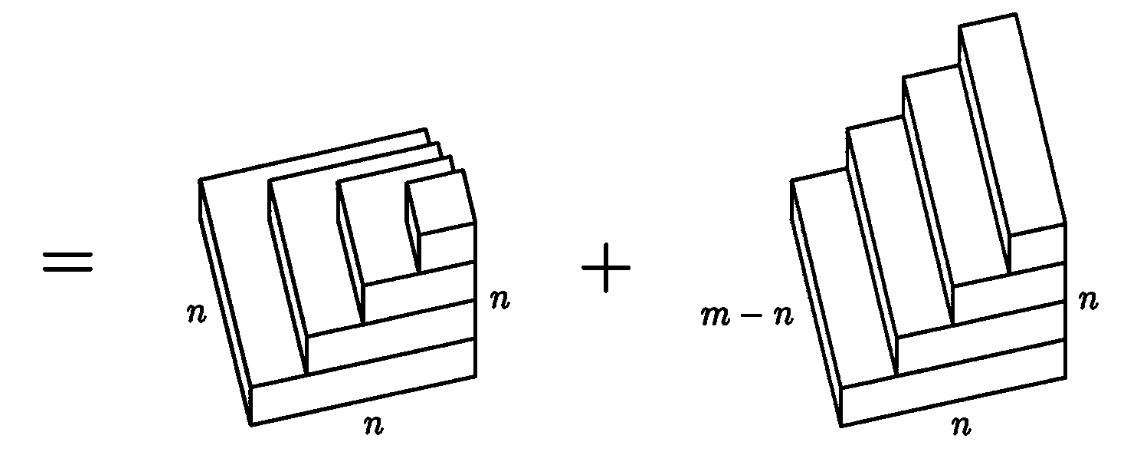
\includegraphics[width=0.8\textwidth]{figures/10-5.png}
\end{figure}
%────────────────────────────────────────
The solid on the left has the shape of a ziggurat and converges to a pyramid as $n \rightarrow \infty$, with volume $\frac{1}{3} n^3$. The solid on the right has the shape of a staircase and converges to a prism as $m, n \rightarrow \infty$, with volume $\frac{1}{2}(m-n) n^2$. Combined, the volume is $\sim \frac{1}{2} m n^2-\frac{1}{6} n^3$. Multiplying by four flops per unit volume, we find

\begin{corollary}
     Work for Householder orthogonalization: $ \sim 2 m n^2-\frac{2}{3} n^3$  flops. 
\end{corollary}